\section{Linear Programming}

\subsection{The Duality Theorem}

	A linear program (LP) asks us to optimize a linear function over a set cut out by finitely many linear inequalities. The duality theorem lets us pair every LP (the \textit{primal}) with a second LP (the \textit{dual}) whose optimal value is the same, and it is the source of both optimality certificates and of the simplex method below. The route to it goes through a sequence of ``theorems of the alternative'' that characterize when a vector lies in the span of some generators, first with arbitrary coefficients (equalities), and then with nonnegative coefficients (inequalities). 

	Given vectors $v_1, \ldots, v_m \in V$, we know that $v \in \Span\{v_i\}$ if $v$ can be written as a linear combination of the $v_i$'s. We wish to formulate an equivalent condition in terms of the dual space. 

	\begin{lemma}[Dual Formulation of Span]
		Let $V$ be a vector space, with $v_1, \ldots, v_m \in V$. For any $v \in V$, the following are equivalent. 
		\begin{enumerate}
		  \item \textit{Primal}. $v \in \Span\{v_i\}$ 
			\item \textit{Dual}. For every $\ell \in V^\dagger$ satisfying $\ell(v_i) = 0$ for all $i$, it is the case that $\ell(v) = 0$. 
		\end{enumerate}
	\end{lemma}
	\begin{proof}
	  We prove bidirectionally. 
		\begin{enumerate}
			\item $(\rightarrow)$. This is easy. Let $v \in \Span\{v_i\}$. Then, if $\ell(v_i) = 0$ for all $i$, then 
				\begin{equation}
					\ell(v) = \ell \bigg( \sum_{i=1}^m a_i v_i \bigg) = \sum_{i=1}^m a_i \ell(v_i) = \sum_{i=1}^m 0 = 0
				\end{equation}

			\item $(\leftarrow)$. We prove the contrapositive. Let $W = \Span\{v_i\}$ and $v \not\in W$. Since $W \cap \Span\{v\} = \{0\}$, we can take their direct sum $W \oplus \Span\{v\}$ and define the linear functional 
				\begin{equation}
					\ell: W \oplus \Span\{v\} \to \mathbb{F}, \quad \ell(w + av) = a
				\end{equation}
				Then, $\ell \in W^\perp$ and $\ell(v) = 1$. We can extend the domain linearly---which is always possible by extending a basis of $W \oplus \Span\{v\}$ to a basis of $V$---to create a functional $\ell \in V^\dagger$. 
		\end{enumerate}
	\end{proof}

	Now, we state a theorem that allows us to check if a vector $v$ can be written as a \textit{nonnegative} linear combination of the $v_i$'s. We need the separating hyperplane theorem first. 

	\begin{theorem}[Separating Hyperplane Theorem]
		Let $C \subset \mathbb{R}^n$ be a nonempty closed convex set, and let $v \in \mathbb{R}^n \setminus C$. Then there exists a nonzero linear functional $\ell \in (\mathbb{R}^n)^\dagger$ and $\alpha \in \mathbb{R}$ such that
		\begin{equation}
			\ell(v) < \alpha \leq \ell(c)
			\qquad \forall c \in C.
		\end{equation}
		Equivalently, there exists a hyperplane
		\begin{equation}
			H = \{x \in \mathbb{R}^n \colon \ell(x) = \alpha\}
		\end{equation}
		that strictly separates $v$ from $C$.
	\end{theorem}
	\begin{proof}
		Since $C$ is nonempty and closed, there exists a point $p \in C$ minimizing the Euclidean distance to $v$, i.e.
		\begin{equation}
			\|v-p\| = \inf_{c \in C} \|v-c\|.
		\end{equation}
		Furthermore, since $v \notin C$, we have $p \neq v$. For any $c \in C$ and $t \in [0,1]$, convexity implies
		\begin{equation}
			p + t(c-p) = (1-t)p + tc \in C.
		\end{equation}
		By the minimality of $p$, we have
		\begin{equation}
			\|v-p\|^2 \leq \|v-p-t(c-p)\|^2.
		\end{equation}
		Expanding the right-hand side gives
		\begin{align}
			\|v-p\|^2 &\leq \|v-p\|^2 - 2t\langle v-p,c-p\rangle + t^2\|c-p\|^2.
		\end{align}
		Subtracting $\|v-p\|^2$ and dividing by $t>0$,
		\begin{equation}
			2\langle v-p,c-p\rangle \leq t\|c-p\|^2.
		\end{equation}
		Taking $t \to 0^+$, we obtain
		\begin{equation}
			\langle v-p,c-p\rangle \leq 0 \qquad \forall c \in C.
		\end{equation}

		Now define the linear functional
		\begin{equation}
			\ell: \mathbb{R}^n \to \mathbb{R}, \qquad \ell(x) = \langle p-v,x\rangle.
		\end{equation}
		Since $p \neq v$, this functional is nonzero. Furthermore, the preceding inequality implies
		\begin{equation}
			\ell(c) \geq \ell(p) \qquad \forall c \in C.
		\end{equation}
		On the other hand,
		\begin{align}
			\ell(p) - \ell(v)
			&= \langle p-v,p-v\rangle \\
			&= \|p-v\|^2 \\
			&> 0.
		\end{align}
		Therefore, setting $\alpha = \ell(p)$, we have
		\begin{equation}
			\ell(v) < \alpha \leq \ell(c)
			\qquad \forall c \in C,
		\end{equation}
		as desired.
	\end{proof}

	\begin{theorem}[Dual Formulation of Positive Span]
		Let $V = \mathbb{R}^n$, with $v_1, \ldots, v_m \in V$. For any $v \in V$, the following are equivalent. 
		\begin{enumerate}
			\item \textit{Primal}. There exists $a_i \geq 0$, $i = 1, \ldots, m$ such that 
				\begin{equation}
					v = \sum_{i=1}^m a_i v_i, \quad a_i \geq 0
				\end{equation}
			\item \textit{Dual}. For every $\ell \in V^\dagger$ satisfying $\ell(v_i) \geq 0$ for all $i$, it is the case that 
				\begin{equation}
					\ell(v) \geq 0
				\end{equation}
		\end{enumerate}

		\begin{figure}[H]
			\centering
			\begin{subfigure}[b]{0.48\textwidth}
				\centering
				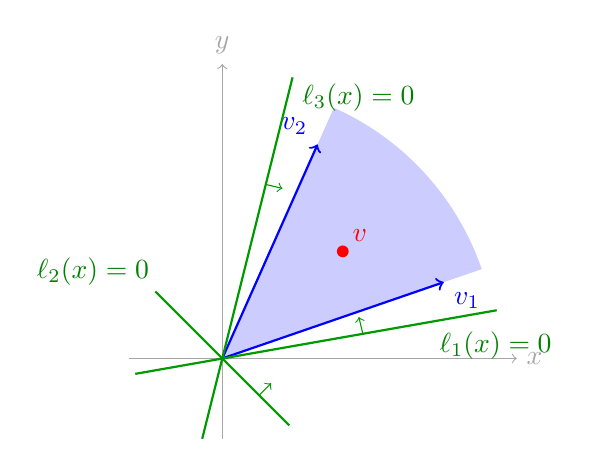
\begin{tikzpicture}[scale=0.85]
					% Axes
					\draw[gray!70, ->] (-1.4,0) -- (4.4,0) node[right] {$x$};
					\draw[gray!70, ->] (0,-1.2) -- (0,4.4) node[above] {$y$};

					% Cone
					\coordinate (O) at (0,0);
					\fill[blue!20] (O) -- (19:4.1)
						arc[start angle=19, end angle=66, radius=4.1] -- cycle;

					\draw[blue, thick, ->] (O) -- (19:3.5)
						node[below right] {$v_1$};
					\draw[blue, thick, ->] (O) -- (66:3.5)
						node[above left] {$v_2$};

					% Point inside cone
					\fill[red] (1.8,1.6) circle (2.5pt);
					\node[red, above right] at (1.8,1.6) {$v$};

					% Functional 1: flatter than v1
					\draw[green!60!black, thick]
						(-1.3,-0.23) -- (4.1,0.72);
					\node[green!50!black, below right] at (3.1,0.55)
						{$\ell_1(x)=0$};
					\draw[green!60!black, ->]
						(2.1,0.37) -- (2.04,0.62);

					% Functional 2: slope -1
					\draw[green!60!black, thick]
						(-1.0,1.0) -- (1.0,-1.0);
					\node[green!50!black, above left] at (-0.95,0.95)
						{$\ell_2(x)=0$};
					\draw[green!60!black, ->]
						(0.55,-0.55) -- (0.73,-0.37);

					% Functional 3: steeper than v2
					\draw[green!60!black, thick]
						(-0.30,-1.2) -- (1.05,4.2);
					\node[green!50!black, right] at (1.05,3.9)
						{$\ell_3(x)=0$};
					\draw[green!60!black, ->]
						(0.65,2.6) -- (0.90,2.54);
				\end{tikzpicture}
				\caption{$v \in \operatorname{cone}(v_1,v_2)$.}
			\end{subfigure}
			\hfill
			\begin{subfigure}[b]{0.48\textwidth}
				\centering
				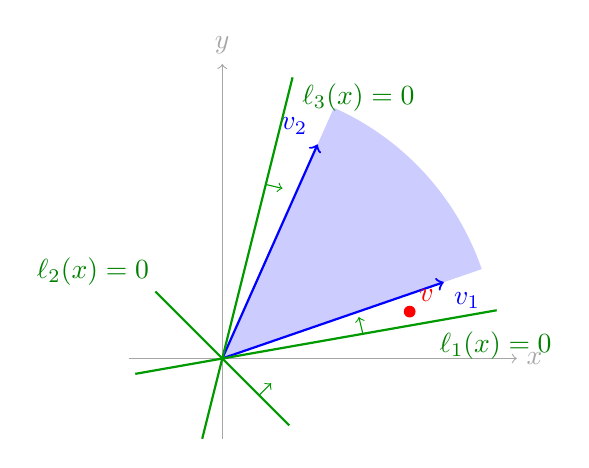
\begin{tikzpicture}[scale=0.85]
					% Axes
					\draw[gray!70, ->] (-1.4,0) -- (4.4,0) node[right] {$x$};
					\draw[gray!70, ->] (0,-1.2) -- (0,4.4) node[above] {$y$};

					% Cone
					\coordinate (O) at (0,0);
					\fill[blue!20] (O) -- (19:4.1)
						arc[start angle=19, end angle=66, radius=4.1] -- cycle;

					\draw[blue, thick, ->] (O) -- (19:3.5)
						node[below right] {$v_1$};
					\draw[blue, thick, ->] (O) -- (66:3.5)
						node[above left] {$v_2$};

					% Point outside cone, between v1 and l1
					\fill[red] (2.8,0.70) circle (2.5pt);
					\node[red, above right] at (2.8,0.70) {$v$};

					% Functional 1: flatter than v1
					\draw[green!60!black, thick]
						(-1.3,-0.23) -- (4.1,0.72);
					\node[green!50!black, below right] at (3.1,0.55)
						{$\ell_1(x)=0$};
					\draw[green!60!black, ->]
						(2.1,0.37) -- (2.04,0.62);

					% Functional 2: slope -1
					\draw[green!60!black, thick]
						(-1.0,1.0) -- (1.0,-1.0);
					\node[green!50!black, above left] at (-0.95,0.95)
						{$\ell_2(x)=0$};
					\draw[green!60!black, ->]
						(0.55,-0.55) -- (0.73,-0.37);

					% Functional 3: steeper than v2
					\draw[green!60!black, thick]
						(-0.30,-1.2) -- (1.05,4.2);
					\node[green!50!black, right] at (1.05,3.9)
						{$\ell_3(x)=0$};
					\draw[green!60!black, ->]
						(0.65,2.6) -- (0.90,2.54);
				\end{tikzpicture}
				\caption{$v \notin \operatorname{cone}(v_1,v_2)$.}
			\end{subfigure}
			\caption{Geometric illustration of the dual characterization
			of positive span. The green lines represent kernels of linear
			functionals, with arrows indicating their nonnegative half-planes.}
			\label{fig:dual_positive_span}
		\end{figure}
	\end{theorem}
	\begin{proof}
		We prove bidirectionally. 
		\begin{enumerate}
		  \item $(\rightarrow)$. Let us have such an $\ell \in V^\dagger$ satisfying $\ell(v_i) \geq 0$. Then, 
				\begin{equation}
					\ell(v) = \ell \bigg( \sum_{i=1}^m a_i v_i \bigg) = \sum_{i=1}^m a_i \ell(v_i) \geq 0
				\end{equation}
				since $a_i \geq 0$ and $\ell(v_i) \geq 0$. 

		  \item $(\leftarrow)$. We would like to prove the contrapositive. Let 
				\begin{equation}
					C = \bigg\{\sum_{i=1}^m a_i v_i \colon a_i \geq 0\bigg\}
				\end{equation}
				by the cone spanned by $v_i$. If $v \not\in C$, then we have to show there exists a $\ell \in V^\dagger$ satisfying $\ell(v_i) \geq 0$ but $\ell(v) < 0$. From the visual, we basically want to construct a small hyperplane squeezed in between the cone and $v$ such that $\ell(v) < 0$. We note three things. 
				\begin{enumerate}
				  \item $C$ is convex since given two vectors $u = \sum_i a_i v_i$ and $w = \sum_i b_i v_i$, we can see that 
						\begin{equation}
						  tu + (1 - t)w = \sum_i (ta_i + (1 - t)b_i) v_i \in C
						\end{equation}
					\item $C$ is a cone, i.e. $tu \in C$ for $t \geq 0, u \in C$. 
					\item $C$ is closed. This is the hard part. Note that a point $u \in C$ can have multiple representations $u = \sum_{i=1}^m a_i v_i$, $a_i \geq 0$. We select one minimizing $A = \sum_{i=1}^m a_i$. Such a minimizer exists since given any feasible representation with coefficient sum $M$, we can restrict the search to 
						\begin{equation}
							S = \bigg\{ a \in \mathbb{R}^m_{\geq 0} \colon \sum_i a_i v_i = u, \sum_i a_i \leq M \bigg\}
						\end{equation}
						This is clearly bounded by $[0, M]^m$, and it is closed since we can define the continuous linear map 
						\begin{equation}
							T: \mathbb{R}^m \to \mathbb{R}^n, T(a) = \sum_{i=1}^m a_i v_i
						\end{equation}
						Therefore, 
						\begin{equation}
							S = T^{-1}(\{u\}) \cap \mathbb{R}^m_{\geq 0} \cap \bigg\{ a \in \mathbb{R}^m \colon \sum_{i=1}^m a_i \leq M \bigg\}
						\end{equation}
						which is a finite intersection of closed sets and hence closed. By Heine-Borel, it is compact. Therefore, by the extreme value theorem, we can find such a minimizer. Now we take a convergence sequence $(u_n) \in C$ such that $u_n \to u$. We are done if we can prove $u \in C$. We do this by first choosing a minimal representation for each $u_n$: 
						\begin{equation}
							u_n = \sum_{i=1}^m a_{n, i} v_i, \quad A_n = \sum_{i=1}^m a_{n, i}
						\end{equation}
						We claim that $(A_n)$ is bounded. Suppose it isn't. Then, by passing to a subsequence, we can assume that $A_n \to \infty$. Because $u_n \to u$, $(u_n)$ is bounded, so 
						\begin{equation}
							\frac{u_n}{A_n} \to 0 
						\end{equation}
						But 
						\begin{equation}
							\frac{u_n}{A_n} = \sum_{i=1}^m \underbrace{\frac{a_{n, i}}{A_n}}_{q_{n, i}} v_i, \quad q_{n, i} \geq 0, \sum_{i=1}^m q_{n, i} = 1
						\end{equation}
						Therefore, the vectors $(q_{n, 1}, \ldots q_{n, m})$ lie in the standard simplex 
						\begin{equation}
							\Delta^{m-1} = \bigg\{ q \in \mathbb{R}^m \colon q_i \geq 0, \sum_i q_i = 1 \bigg\}
						\end{equation}
						Since this simplex is compact, there exists a subsequence along which $q_{n, i} \to q_i$ for every $i$; we relabel it by $n$. Passing to the limit gives 
						\begin{equation}
							\sum_{i=1}^m q_i v_i = 0, \quad q_i \geq 0, \sum_{i=1}^m q_i = 1
						\end{equation}

						Since $\sum_{i=1}^m q_i = 1$, there exists some $j$ such that $q_j > 0$. Furthermore, for every $i$ such that $q_i > 0$, we have $q_{n,i} \to q_i > 0$, and hence $a_{n,i} = A_n q_{n,i} > 0$ for sufficiently large $n$.

						Now define
						\begin{equation}
							t_n = \min_{i \colon q_i > 0} \frac{a_{n,i}}{q_i} > 0.
						\end{equation}
						Consider the new coefficients
						\begin{equation}
							a_{n,i}^{\prime} = a_{n,i} - t_n q_i.
						\end{equation}
						By the definition of $t_n$, we have $a_{n,i}^{\prime} \geq 0$ for all $i$. Furthermore,
						\begin{align}
							\sum_{i=1}^m a_{n,i}^{\prime} v_i
							&= \sum_{i=1}^m (a_{n,i} - t_n q_i)v_i \\
							&= u_n - t_n \sum_{i=1}^m q_i v_i \\
							&= u_n.
						\end{align}
						Therefore, $(a_{n,i}^{\prime})$ is another nonnegative representation of $u_n$. However,
						\begin{align}
							\sum_{i=1}^m a_{n,i}^{\prime}
							&= \sum_{i=1}^m a_{n,i}
								- t_n \sum_{i=1}^m q_i \\
							&= A_n - t_n \\
							&< A_n,
						\end{align}
						contradicting the minimality of $A_n$. Therefore, $(A_n)$ must be bounded.

						Since $0 \leq a_{n,i} \leq A_n$ for all $i$, the sequence of coefficient vectors $(a_{n,1},\ldots,a_{n,m})$ is bounded in $\mathbb{R}^m$. By Bolzano-Weierstrass, there exists a convergent subsequence such that
						\begin{equation}
							a_{n,i} \to a_i \geq 0
							\qquad \forall i.
						\end{equation}
						Taking the limit in
						$u_n = \sum_{i=1}^m a_{n,i}v_i$ gives
						\begin{equation}
							u = \sum_{i=1}^m a_i v_i \in C.
						\end{equation}
						Therefore, $C$ is sequentially closed, and hence closed in $\mathbb{R}^n$.
				\end{enumerate}

				Since we have shown that $C$ is a closed convex cone, by the separating hyperplane theorem, there exists a nonzero linear functional $\ell \in V^\dagger$ and $\alpha \in \mathbb{R}$ such that
				\begin{equation}
					\ell(v) < \alpha \leq \ell(c)
					\qquad \forall c \in C.
				\end{equation}
				Since $0 \in C$, we have
				\begin{equation}
					\ell(v) < \alpha \leq \ell(0) = 0,
				\end{equation}
				and hence $\ell(v) < 0$. We claim that $\ell(c) \geq 0$ for all $c \in C$. Suppose otherwise, so that there exists $c \in C$ with $\ell(c) < 0$. Since $C$ is a cone, $tc \in C$ for every $t \geq 0$. Thus,
				\begin{equation}
					t\ell(c) = \ell(tc) \geq \alpha
					\qquad \forall t \geq 0.
				\end{equation}
				Taking $t \to \infty$ gives a contradiction, since $t\ell(c) \to -\infty$. Therefore, $\ell(c) \geq 0$ for all $c \in C$. In particular, since $v_i \in C$,
				\begin{equation}
					\ell(v_i) \geq 0 \quad \forall i,
					\qquad \ell(v) < 0.
				\end{equation}

		\end{enumerate}
	\end{proof}

  In the rest of this section, vector inequalities are entry-wise. Elements of $\mathbb{R}^n$ are column vectors, and elements of the dual space $(\mathbb{R}^n)^\dagger$ are row vectors, so that a functional $\lambda$ acts on $r$ by the matrix product $\lambda r$.

	\begin{corollary}[Farkas' Lemma, Equality Form]
		Let $W \in \mathbb{R}^{n \times m}$ be the matrix whose columns are the generators\footnote{Not necessarily linearly independent.} of a cone. For any $r \in \mathbb{R}^n$, the following are equivalent. 
		\begin{enumerate}
			\item \textit{Primal}. There exists an $a \in \mathbb{R}^m$ such that 
				\begin{equation}
				  r = Wa, \quad a \geq 0
				\end{equation} 
				That is, $r$ lies in the \textit{cone} generated by $W$. 

			\item \textit{Dual}. For every row vector $\lambda \in \mathbb{R}^{1 \times n}$ satisfying $\lambda W \geq 0$, it is the case that 
				\begin{equation}
					\lambda r \geq 0
				\end{equation}
		\end{enumerate}
  \end{corollary}
	\begin{proof}
	  Obvious from theorem above. 
	\end{proof}

	Now here is a variant that relaxes the primal condition (the equality $r = Wa$ becomes the inequality $r \geq Wa$). On the dual side, we must now check $\lambda r \geq 0$ only for the $\lambda$ that also satisfy $\lambda \geq 0$. This is a smaller set of $\lambda$'s to check, so the dual condition is weaker, which matches the weaker primal condition. 

	\begin{theorem}[Farkas' Lemma, Inequality Form]
		Let $W \in \mathbb{R}^{n \times m}$ be the matrix whose columns are the generators\footnote{Not necessarily linearly independent.} of a cone. For any $r \in \mathbb{R}^n$, the following are equivalent. 
		\begin{enumerate}
			\item \textit{Primal}. There exists an $a \in \mathbb{R}^m$ such that 
				\begin{equation}
				  r \geq Wa, \quad a \geq 0
				\end{equation}

			\item \textit{Dual}. For every row vector $\lambda \in \mathbb{R}^{1 \times n}$ satisfying $\lambda W \geq 0$ and $\lambda \geq 0$, it is the case that $\lambda r \geq 0$. 
		\end{enumerate}
  \end{theorem}
	\begin{proof}
		We prove bidirectionally.
		\begin{enumerate}
			\item $(\rightarrow)$. Suppose there exists $a \geq 0$ such that $r \geq Wa$. For every $\lambda \geq 0$ satisfying $\lambda W \geq 0$, we have
				\begin{equation}
					\lambda r \geq \lambda Wa \geq 0.
				\end{equation}

			\item $(\leftarrow)$. Suppose that for every $\lambda \geq 0$ satisfying $\lambda W \geq 0$, we have $\lambda r \geq 0$. Observe that the primal condition can be rewritten by introducing a slack variable
				$s \in \mathbb{R}^n_{\geq 0}$:
				\begin{align}
					r \geq Wa,\quad a \geq 0
					&\iff r = Wa + s,\quad a,s \geq 0 \\
					&\iff
					r = \begin{pmatrix} W & I_n \end{pmatrix}
					\begin{pmatrix} a \\ s \end{pmatrix},
					\quad
					\begin{pmatrix} a \\ s \end{pmatrix} \geq 0.
				\end{align}
				Define the augmented matrix
				\begin{equation}
					\widetilde{W}
					= \begin{pmatrix} W & I_n \end{pmatrix}
					\in \mathbb{R}^{n \times (m+n)}.
				\end{equation}
				By the dual formulation of positive span, there exists a nonnegative coefficient vector $b$ satisfying $r = \widetilde{W}b$ if and only if
				\begin{equation}
					\lambda \widetilde{W} \geq 0 \implies \lambda r \geq 0
				\end{equation}
				for every $\lambda \in \mathbb{R}^{1 \times n}$. But
				\begin{align}
					\lambda \widetilde{W} \geq 0
					&\iff
					\begin{pmatrix}
						\lambda W & \lambda I_n
					\end{pmatrix} \geq 0 \\
					&\iff \lambda W \geq 0,\quad \lambda \geq 0.
				\end{align}
				By assumption, every such $\lambda$ satisfies $\lambda r \geq 0$. Therefore, there exists $b \geq 0$ such that
				\begin{equation}
					r = \widetilde{W}b.
				\end{equation}
				Writing $b = (a^\top,s^\top)^\top$, we obtain
				\begin{equation}
					r = Wa + s,\qquad a,s \geq 0.
				\end{equation}
				Hence $r \geq Wa$ with $a \geq 0$. 
		\end{enumerate}
	\end{proof}

	\begin{definition}[Primal and Dual Feasibility]
		\label{def:primal_dual}
		Let $W \in \mathbb{R}^{n \times m}$, $r \in \mathbb{R}^n$, and $p \in \mathbb{R}^{1 \times m}$. Consider the following two optimization problems.
		\begin{enumerate}
			\item \textit{Primal}. The \textbf{primal problem} is
				\begin{equation}
					S = \sup_{a \in \mathbb{R}^m} \{pa \colon Wa \leq r,\; a \geq 0\}.
				\end{equation}
				A vector $a \in \mathbb{R}^m$ satisfying $Wa \leq r,\qquad a \geq 0$ is called \textbf{primal feasible}.

			\item \textit{Dual}. The \textbf{dual problem} is
				\begin{equation}
					s = \inf_{\lambda \in \mathbb{R}^{1 \times n}} \{\lambda r \colon \lambda W \geq p,\; \lambda \geq 0\}.
				\end{equation}
				A row vector $\lambda \in \mathbb{R}^{1 \times n}$ satisfying $\lambda W \geq p,\qquad \lambda \geq 0$ is called \textbf{dual feasible}.
		\end{enumerate}
		For each problem, if the feasible set is nonempty, then the problem is called \textbf{feasible}. 
	\end{definition}

	In case the motivation is still not clear, we can do a manual derivation of the dual from the primal. 

  \begin{example}[Manual Derivation of Dual from Primal]
		Given a primal problem such as 
    \begin{equation}
      \max{2x + y} \text{ subject to } \begin{cases} x + y \leq 3 \\ x - y \leq 1 \\ x, y \geq 0 \end{cases} 
    \end{equation}
    we can just find \textit{one} solution satisfying the constraints and use it as a lower bound on the optimum. Say we find one, e.g. $x = y = 0$, which does satisfy all constraints. Now if we want to find an \textit{upper bound} on the value of the solution, we can use duality. We create new variables $a, b \geq 0$, and observe that 
    \begin{align}
      x + y \leq 3 & \implies a (x + y) \leq 3a \\
      x - y \leq 1 & \implies b (x - y) \leq b
    \end{align}
    Thus by adding the two we have $(a + b) x + (a - b) y \leq 3a + b$. 

    Now if we suppose $a + b \geq 2$ and $a - b \geq 1$ (which are the coeffients of $2x + y$), then since $x, y \geq 0$, we have 
    \begin{equation}
      2x + y \leq (a + b) x + (a - b) y \leq 3a + b
    \end{equation} 
    so any $a, b$ satisfying the above inequalities give an upper bound of $3a + b$ on the value of the optimal solution. Say we have $a = 2, b = 1$, which does satisfy. Then $3a + b = 7$ is an upper bound of $2x + y$. Therefore, to get the tightest upper bound, we can minimize the dual problem 
    \begin{equation}
      \min{3a + b} \text{ subject to } \begin{cases} a + b \geq 2 \\ a - b \geq 1 \\ a, b \geq 0 \end{cases}
    \end{equation}
  \end{example}

	It should be clear from our line of results that point that we wish to make is that the primal and dual are two reformulations of the same problem, and by solving one, we can solve the other. 

	\begin{lemma}[Dual of Dual is Primal]
	  Given the primal and dual problems above, 
		\begin{equation}
			S = \sup_{a \in \mathbb{R}^m} \{pa \colon Wa \leq r,\; a \geq 0\}, \quad s = \inf_{\lambda \in \mathbb{R}^{1 \times n}} \{\lambda r \colon \lambda W \geq p,\; \lambda \geq 0\}.
		\end{equation}
		we can reformulate the dual problem as a primal problem, and the dual of the dual is the primal. 
	\end{lemma}
	\begin{proof}
	  Let $\nu = \lambda^T$. Then, we can reformulate the dual as a primal problem
		\begin{align}
			s & = \inf_{\nu \in \mathbb{R}^n} \{r^T \nu \colon W^T \nu \geq p^T, \nu \geq 0 \} \\ 
				& = \sup_{\nu \in \mathbb{R}^n} \{ (-r)^T \nu : (-W)^T \nu \leq (-p)^T, \nu \geq 0 \}
		\end{align}
		The dual of this is 
		\begin{equation}
			\inf_{\phi \in \mathbb{R}^{1 \times n}} \{\phi (-p)^T \colon \phi (-W)^T \geq (-r)^T , \phi \geq 0 \}
		\end{equation}
		We can reformulate it as a primal again, and substituting $\mu = \phi^T$ gives us 
		\begin{equation}
			\sup_{\phi \in \mathbb{R}^{1 \times n}} \{\phi p^T \colon W \phi^T \leq r, \phi \geq 0 \} = \sup_{\mu \in \mathbb{R}^n} \{p \mu \colon W \mu \leq r, \mu \geq 0 \}
		\end{equation}
		which is exactly the first primal problem. 
	\end{proof}

	\begin{lemma}[Weak Duality]
		Let $W \in \mathbb{R}^{n \times m}$, $r \in \mathbb{R}^n$, and $p \in \mathbb{R}^{1 \times m}$. For any primal feasible vector $a$ and dual feasible vector $\lambda$, we have
		\begin{equation}
			pa \leq \lambda r.
		\end{equation}
		Consequently, if both problems are feasible,
		\begin{equation}
			S \leq s.
		\end{equation}
	\end{lemma}
	\begin{proof}
		Since $\lambda W \geq p$ and $a \geq 0$,
		\begin{equation}
			pa \leq \lambda Wa.
		\end{equation}
		Furthermore, since $Wa \leq r$ and $\lambda \geq 0$,
		\begin{equation}
			\lambda Wa \leq \lambda r.
		\end{equation}
		Combining these inequalities gives
		\begin{equation}
			pa \leq \lambda Wa \leq \lambda r.
		\end{equation}
		Taking the supremum over all primal feasible $a$ and the infimum over all dual feasible $\lambda$ gives $S \leq s$.
	\end{proof}

	Now, we can establish the equivalence of the primal and dual problems. 

	\begin{theorem}[Strong Duality]
		Let $W \in \mathbb{R}^{n \times m}$, $r \in \mathbb{R}^n$, and $p \in \mathbb{R}^{1 \times m}$, with the conventions $\sup \emptyset = -\infty$ and $\inf \emptyset = +\infty$. Then exactly one of the following holds. 
		\begin{enumerate}
			\item Both optimal values are finite and attained, i.e. there exist a primal feasible vector $a^\ast$ and a dual feasible vector $\lambda^\ast$ such that
				\begin{equation}
					pa^\ast = S = s = \lambda^\ast r.
				\end{equation}
			\item The primal is feasible and unbounded ($S = +\infty$), and the dual is infeasible. 
			\item The dual is feasible and unbounded ($s = -\infty$), and the primal is infeasible. 
			\item Both problems are infeasible. 
		\end{enumerate}
		In particular, if either problem has a finite optimal value, so does the other. 
	\end{theorem}
	\begin{proof}
		The four cases correspond to the four combinations of feasibility, so we treat each. 

		\begin{enumerate}
			\item \textit{Both feasible}. Fix a primal feasible $a_0$ and a dual feasible $\lambda_0$. We claim that there exist $a \geq 0$ and $\nu \geq 0$ (a column vector, $\nu = \lambda^\top$) such that 
				\begin{equation}
					Wa \leq r, \qquad -W^\top \nu \leq -p^\top, \qquad -pa + r^\top \nu \leq 0.
				\end{equation}
				That is, $a$ is primal feasible, $\lambda = \nu^\top$ is dual feasible, and $pa \geq \lambda r$. Given this claim, weak duality gives $pa \leq S \leq s \leq \lambda r$, and combined with $pa \geq \lambda r$ all of these are equalities. Hence $S = s$ is finite and attained at $a^\ast = a$ and $\lambda^\ast = \lambda$. 

				To prove the claim, write the system as $Mz \leq b$ with $z = (a, \nu) \geq 0$, where 
				\begin{equation}
					M = \begin{pmatrix} W & 0 \\ 0 & -W^\top \\ -p & r^\top \end{pmatrix}, \qquad 
					b = \begin{pmatrix} r \\ -p^\top \\ 0 \end{pmatrix}.
				\end{equation}
				By Farkas' lemma (inequality form), such a $z$ exists if and only if every row vector $y = (y_1, y_2, t) \geq 0$, with $y_1 \in \mathbb{R}^{1 \times n}$, $y_2 \in \mathbb{R}^{1 \times m}$, $t \in \mathbb{R}$, satisfying $yM \geq 0$ also satisfies $yb \geq 0$. Computing, 
				\begin{equation}
					yM \geq 0 \iff y_1 W \geq tp \;\text{ and }\; W y_2^\top \leq t r, \qquad yb = y_1 r - p y_2^\top.
				\end{equation}
				Let $y \geq 0$ satisfy the left-hand conditions. There are two cases. 
				\begin{itemize}
					\item $t > 0$. Dividing by $t$, the vector $\lambda = y_1/t$ is dual feasible and $a = y_2^\top/t$ is primal feasible. By weak duality, $pa \leq \lambda r$, and multiplying by $t$ gives $y_1 r - p y_2^\top \geq 0$. 
					\item $t = 0$. Then $y_1 W \geq 0$ and $W y_2^\top \leq 0$. Using $y_1 \geq 0$, $Wa_0 \leq r$, $a_0 \geq 0$,
						\begin{equation}
							y_1 r \geq y_1 W a_0 \geq 0.
						\end{equation}
						Using $y_2 \geq 0$, $\lambda_0 W \geq p$, $\lambda_0 \geq 0$,
						\begin{equation}
							p y_2^\top \leq \lambda_0 W y_2^\top \leq 0.
						\end{equation}
						Together, $y_1 r - p y_2^\top \geq 0$.
				\end{itemize}
				This proves the claim. 

			\item \textit{Primal feasible, dual infeasible}. That the dual is infeasible means there is no $\nu \geq 0$ with $-W^\top \nu \leq -p^\top$. By Farkas' lemma (inequality form) applied to the matrix $-W^\top$ and the vector $-p^\top$, there exists a row vector $y \geq 0$ with $-yW^\top \geq 0$ and $-yp^\top < 0$. Setting $d = y^\top \in \mathbb{R}^m$, this says $d \geq 0$, $Wd \leq 0$, and $pd > 0$. For a primal feasible $a_0$ and any $\tau \geq 0$, the vector $a_0 + \tau d$ is primal feasible, since $W(a_0 + \tau d) \leq Wa_0 \leq r$. Its objective value is $pa_0 + \tau pd \to \infty$, so $S = +\infty$. 

			\item \textit{Dual feasible, primal infeasible}. That the primal is infeasible means there is no $a \geq 0$ with $Wa \leq r$. By Farkas' lemma (inequality form) applied directly, there exists $\lambda \geq 0$ with $\lambda W \geq 0$ and $\lambda r < 0$. For a dual feasible $\lambda_0$ and any $\tau \geq 0$, the vector $\lambda_0 + \tau \lambda$ is dual feasible, and its objective value is $\lambda_0 r + \tau \lambda r \to -\infty$, so $s = -\infty$. 

			\item \textit{Both infeasible}. Nothing to prove. 
		\end{enumerate}
		The four cases are mutually exclusive since they have distinct feasibility patterns. 
	\end{proof}

	\begin{corollary}[Primal-Dual Optimality Criterion]
		A primal feasible vector $a^\ast$ and a dual feasible vector $\lambda^\ast$ are both optimal if and only if
		\begin{equation}
			pa^\ast = \lambda^\ast r.
		\end{equation}
	\end{corollary}
	\begin{proof}
		We prove bidirectionally. 
		\begin{enumerate}
			\item $(\rightarrow)$. By strong duality,
				\begin{equation}
					pa^\ast = S = s = \lambda^\ast r.
				\end{equation}
			\item $(\leftarrow)$. By weak duality, for any primal feasible $a$ and dual feasible $\lambda$,
				\begin{equation}
					pa \leq \lambda^\ast r
					= pa^\ast \leq \lambda r.
				\end{equation}
			Therefore, $a^\ast$ maximizes the primal objective and $\lambda^\ast$ minimizes the dual objective.
		\end{enumerate}
	\end{proof}

	Weak duality is elementary and follows directly from the inequalities. Strong duality is the substantial theorem, and it is exactly where Farkas' lemma is needed. Note that the optimality criterion above is a \textit{certificate}: to prove that a feasible $a^\ast$ is optimal, it suffices to exhibit a dual feasible $\lambda^\ast$ with the same objective value.

	\begin{example}[Production Planning and Resource Pricing]
		Suppose a furniture factory produces tables and chairs. Each table requires $2$ units of wood and $1$ hour of labor, generating a profit of $\$50$. Each chair requires $1$ unit of wood and $2$ hours of labor, generating a profit of $\$40$. The factory has $100$ units of wood and $80$ hours of labor available.

		Let $a_1,a_2 \geq 0$ denote the quantities of tables and chairs produced, respectively. We define
		\begin{equation}
			W = \begin{pmatrix}
				2 & 1 \\
				1 & 2
			\end{pmatrix}, \qquad
			r = \begin{pmatrix}
				100 \\ 80
			\end{pmatrix}, \qquad
			p = \begin{pmatrix}
				50 & 40
			\end{pmatrix}.
		\end{equation}

		\begin{enumerate}
			\item \textit{Primal}. The factory wishes to maximize its profit subject to its resource constraints:
				\begin{equation}
					S = \sup_{a \geq 0}
					\{pa \colon Wa \leq r\}.
				\end{equation}
				Equivalently,
				\begin{align}
					\text{maximize} \quad &50a_1 + 40a_2 \\
					\text{subject to} \quad
					&2a_1 + a_2 \leq 100, \\
					&a_1 + 2a_2 \leq 80, \\
					&a_1,a_2 \geq 0.
				\end{align}

			\item \textit{Dual}. Let $\lambda_1,\lambda_2 \geq 0$ represent the implicit prices of wood and labor.\footnote{Suppose a buyer wants to purchase all your wood and labor instead of letting you make furniture. What is the lowest price the buyer could offer that you would still accept? Let $\lambda_1$ be the price per unit of wood and $\lambda_2$ the price per hour of labor. The buyer's total cost is $100 \lambda_1 + 80 \lambda_2$ and the buyer wants to minimize it. This is the dual objective. You would refuse any offer that pays less than you could earn by making furniture. A table uses 2 wood and 1 labor hour and earns \$50, so you need $2 \lambda_1 + \lambda_2 \geq 50$. A chair needs $\lambda_1 + 2\lambda_2 \geq 40$. These are the dual constraints $\lambda W \geq p$. Prices can't be negative, which gives $\lambda \geq 0$. } The total resource value required to produce each product must be at least its profit. Therefore,
				\begin{equation}
					s = \inf_{\lambda \geq 0}
					\{\lambda r \colon \lambda W \geq p\}.
				\end{equation}
				Equivalently,
				\begin{align}
					\text{minimize} \quad &100\lambda_1 + 80\lambda_2 \\
					\text{subject to} \quad
					&2\lambda_1 + \lambda_2 \geq 50, \\
					&\lambda_1 + 2\lambda_2 \geq 40, \\
					&\lambda_1,\lambda_2 \geq 0.
				\end{align}
		\end{enumerate}

		Solving the primal problem gives
		\begin{equation}
			a^* = \begin{pmatrix} 40 \\ 20 \end{pmatrix}, \qquad S = pa^* = 2800.
		\end{equation}
		Solving the dual problem gives
		\begin{equation}
			\lambda^* = \begin{pmatrix} 20 & 10 \end{pmatrix}, \qquad s = \lambda^*r = 2800.
		\end{equation}
		Therefore,
		\begin{equation}
			S = s = 2800,
		\end{equation}
		verifying strong duality.
	\end{example}

	\begin{example}[Primal Feasible, Dual Infeasible]
		An \hyperref[qf-def:arbitrage_portfolio]{arbitrage} is a trading strategy that requires no net investment and cannot lose money, but has a positive profit in at least one outcome. For example, suppose a stock ABC trades at $\$100$, and a European call option on ABC with strike $\$90$ expiring in one year trades at $\$8$. Since the right to buy at $\$90$ a stock worth $\$100$ is worth at least $\$10$, the option is underpriced. Consider the following trade today: buy one call for $\$8$ and short sell one share of ABC for $\$100$, for a net cash inflow of $\$92$. At expiration, with stock price $S_T$, 
		\begin{itemize}
			\item if $S_T \geq 90$, exercise the call, buy the share at $\$90$ and return it to close the short, leaving a profit of $92 - 90 = \$2$;
			\item if $S_T < 90$, let the call expire, buy the share on the market at $S_T$ and return it, leaving a profit of $92 - S_T > \$2$.
		\end{itemize}
		In every outcome we keep at least $\$2$ without having invested anything (ignoring interest). Doing the same trade on $t$ contracts multiplies the profit by $t$. 

		Let 
		\begin{equation}
			W = \begin{pmatrix} 1 & -1 \end{pmatrix}, \qquad r = 1, \qquad p = \begin{pmatrix} 1 & 1 \end{pmatrix},
		\end{equation}
		so that the primal is 
		\begin{align}
			\text{maximize} \quad &a_1 + a_2 \\
			\text{subject to} \quad &a_1 - a_2 \leq 1, \\
			&a_1, a_2 \geq 0.
		\end{align}
		The primal is feasible, since $a = (0, 0)$ satisfies the constraints. It is also unbounded: for any $t \geq 0$, the vector $a = (t, t)$ satisfies $Wa = 0 \leq 1$ and has objective value $2t \to \infty$. 

		The dual, with a single variable $\lambda \geq 0$, is 
		\begin{align}
			\text{minimize} \quad &\lambda \\
			\text{subject to} \quad &\lambda \geq 1, \\
			&-\lambda \geq 1, \\
			&\lambda \geq 0.
		\end{align}
		The first two constraints say $\lambda \geq 1$ and $\lambda \leq -1$, which cannot both hold, so the dual is infeasible. This is case 2 of the strong duality theorem. The vector $d = (1, 1)^\top$ is the direction from the proof: $d \geq 0$, $Wd = 0 \leq 0$, and $pd = 2 > 0$. Moving along $d$ keeps the primal feasible while increasing the objective without bound. Weak duality is consistent with this: it says every dual feasible $\lambda$ gives an upper bound on the primal, and here there is no such $\lambda$, so nothing stops the primal from growing. 
	\end{example}

	\begin{example}[Both Infeasible]
		A problem is \textbf{infeasible} when its constraints contradict each other, so that no choice of variables satisfies all of them at once. This typically happens when constraints come from different sources that nobody checked against each other. For example, suppose a hospital staffs a cardiac ward and a general ward, and let $a_1, a_2$ be the numbers of nurses assigned to each, with the goal of staffing as many nurses as possible ($\max a_1 + a_2$). The nurses' union contract says that the cardiac ward may have at most one more nurse than the general ward, 
		\begin{equation}
			a_1 - a_2 \leq 1,
		\end{equation}
		while a new state safety regulation requires the cardiac ward to have at least two more nurses than the general ward, 
		\begin{equation}
			a_1 - a_2 \geq 2.
		\end{equation}
		No staffing plan satisfies both since adding the contract inequality $a_1 - a_2 \leq 1$ to the regulation written as $-a_1 + a_2 \leq -2$ gives $0 \leq -1$, which is absurd. Every staffing plan breaks one of the two rules, so the problem is infeasible. Let 
		\begin{equation}
			W = \begin{pmatrix} 1 & -1 \\ -1 & 1 \end{pmatrix}, \qquad r = \begin{pmatrix} 1 \\ -2 \end{pmatrix}, \qquad p = \begin{pmatrix} 1 & 1 \end{pmatrix}.
		\end{equation}
		\begin{enumerate}
			\item \textit{Primal}. The constraints $Wa \leq r$ read $a_1 - a_2 \leq 1$ and $-a_1 + a_2 \leq -2$, i.e. $a_1 - a_2 \leq 1$ and $a_1 - a_2 \geq 2$. These contradict each other, so the primal is infeasible. A certificate (from the inequality form of Farkas' lemma) is $\lambda = (1, 1)$, which satisfies $\lambda \geq 0$ and $\lambda W = (0, 0) \geq 0$, but $\lambda r = 1 - 2 = -1 < 0$. 

			\item \textit{Dual}. The constraints $\lambda W \geq p$ with $\lambda \geq 0$ read 
				\begin{equation}
					\lambda_1 - \lambda_2 \geq 1, \qquad -\lambda_1 + \lambda_2 \geq 1.
				\end{equation}
				Adding them gives $0 \geq 2$, so the dual is infeasible. A certificate is $d = (1, 1)^\top$, which satisfies $d \geq 0$, $Wd = (0, 0)^\top \leq 0$, and $pd = 2 > 0$. 
		\end{enumerate}
		This is case 4. With the conventions $\sup \emptyset = -\infty$ and $\inf \emptyset = +\infty$, we get $S = -\infty$ and $s = +\infty$. The two values differ, so strong duality gives no information in this case. Note that the vector $d$ would make the primal unbounded \textit{if} the primal had a feasible point, but it does not. 
	\end{example}

\subsection{Complementary Slackness and Sensitivity}

	Strong duality has two useful consequences. The first tells us exactly how an optimal primal and dual pair must interact. 

	\begin{theorem}[Complementary Slackness]
		Let $a$ be primal feasible and $\lambda$ be dual feasible. Then $a$ and $\lambda$ are both optimal if and only if
		\begin{equation}
			\lambda (r - Wa) = 0 \qquad \text{and} \qquad (\lambda W - p) a = 0.
		\end{equation}
	\end{theorem}
	\begin{proof}
		We have the identity 
		\begin{equation}
			\lambda r - pa = \underbrace{\lambda (r - Wa)}_{\geq 0} + \underbrace{(\lambda W - p) a}_{\geq 0}.
		\end{equation}
		Both terms are nonnegative by feasibility. By the optimality criterion, $a$ and $\lambda$ are both optimal if and only if $\lambda r - pa = 0$, which holds if and only if both nonnegative terms vanish. 
	\end{proof}

	Since every term in these two inner products is nonnegative, this is equivalent to the entrywise statements 
	\begin{align}
		\lambda_i > 0 &\implies (Wa)_i = r_i, \qquad \text{(a priced resource is fully used)}\\
		a_j > 0 &\implies (\lambda W)_j = p_j. \qquad \text{(a produced good has zero profit after pricing)}
	\end{align}

	\begin{example}[Complementary Slackness for Furniture, No Slack]
		For the furniture example above, $a^\ast = (40, 20)^\top$ uses all of the wood and labor, $Wa^\ast = (100, 80)^\top = r$, and $\lambda^\ast W = (50, 40) = p$. So complementary slackness holds with $\lambda^\ast > 0$ and $a^\ast > 0$, with no slack in either place. We can also run this in reverse, to \textit{compute} the dual solution from the primal one. Suppose we have only solved the primal and found $a^\ast = (40, 20)^\top$, and we do not yet know $\lambda^\ast$. Both $a_1^\ast$ and $a_2^\ast$ are positive, so complementary slackness forces both dual constraints to be tight, $(\lambda^\ast W)_j = p_j$ for $j = 1, 2$:
		\begin{align}
			2\lambda_1 + \lambda_2 &= 50, \\
			\lambda_1 + 2\lambda_2 &= 40.
		\end{align}
		This is a $2 \times 2$ linear system, and its solution is $\lambda^\ast = (20, 10)$. It remains to check that this $\lambda^\ast$ is actually dual feasible and optimal: indeed $\lambda^\ast \geq 0$, $\lambda^\ast W = (50, 40) \geq p$, and $\lambda^\ast r = 100 \cdot 20 + 80 \cdot 10 = 2800 = pa^\ast$, so by the optimality criterion $\lambda^\ast$ is optimal. Had a constraint been slack at $a^\ast$ (say $(Wa^\ast)_i < r_i$), complementary slackness would instead give $\lambda_i = 0$, which removes an unknown.
	\end{example}

	In general, if we guess the set $B$ of positive primal variables (the optimal basis in the language of the simplex method below), the equations $(\lambda W)_j = p_j$ for $j \in B$ and $\lambda_i = 0$ for the slack constraints form a linear system for $\lambda^\ast$, which is then verified for feasibility as above.

	The second consequence is that the dual variables are marginal prices. 

	\begin{theorem}[Dual Variables are Maringal/Shadow Prices]
		Suppose the dual is feasible, and let $S(r) = \sup_{a \in \mathbb{R}^m} \{pa \colon Wa \leq r, a \geq 0 \}$ denote the optimal value of the primal as a function of the resource vector $r$, with $W$ and $p$ fixed. Then, 
		\begin{enumerate}
		  \item On the set of $r$ for which the primal is feasible, $S(r)$ is finite, concave, and piecewise linear in $r$. 
			\item If $\lambda^\ast$ is an optimal dual solution for $r$, then 
				\begin{equation}
					S(r') \leq S(r) + \lambda^\ast (r' - r) \qquad \forall r'.
				\end{equation}
				That is, $\lambda^\ast$ is a supergradient of $S$ at $r$. In particular, wherever $S$ is differentiable, $\partial S / \partial r_i = \lambda^\ast_i$. 
		\end{enumerate}
	\end{theorem}
	\begin{proof}
		The dual feasible set $D = \{\lambda \geq 0 \colon \lambda W \geq p\}$ does not depend on $r$. By strong duality, for every $r$ with the primal feasible, 
		\begin{equation}
			S(r) = \inf_{\lambda \in D} \lambda r,
		\end{equation}
		which is a pointwise infimum of linear functions of $r$, and hence concave. It is finite since $D$ and the primal are nonempty, and it is piecewise linear because $D$ is a polyhedron whose infimum is attained at one of its finitely many vertices (it contains no lines since $\lambda \geq 0$). For the supergradient inequality, $\lambda^\ast \in D$ is dual feasible for every $r'$, so $S(r') \leq \lambda^\ast r'$ by weak duality (or $S(r') = -\infty$), while $S(r) = \lambda^\ast r$. Subtracting gives the claim. 
	\end{proof}

	In the furniture example, $\lambda^\ast = (20, 10)$, so one extra unit of wood is worth $\$20$ and one extra hour of labor is worth $\$10$. Indeed with $101$ units of wood, solving the constraints gives $a = (122/3, 59/3)$ and profit $2820 = 2800 + 20$. 

\subsection{Geometry of Linear Programs}

	We now turn to algorithms. For the geometry it is convenient to use the \textbf{standard form}, which is related to the canonical form by adding slack variables. In this subsection (and the next) the notation resets: $A \in \mathbb{R}^{m \times n}$ with $\operatorname{rank} A = m$, $b \in \mathbb{R}^m$, $c \in \mathbb{R}^{1 \times n}$, and the LP is 
	\begin{equation}
		\min \{cx \colon Ax = b,\; x \geq 0\}.
	\end{equation}
	To convert the canonical primal $\max\{pa \colon Wa \leq r, a \geq 0\}$, we introduce slacks $s \geq 0$ with $Wa + s = r$, and set 
	\begin{equation}
		x = \begin{pmatrix} a \\ s \end{pmatrix}, \quad A = \begin{pmatrix} W & I_n \end{pmatrix}, \quad b = r, \quad c = \begin{pmatrix} -p & 0 \end{pmatrix},
	\end{equation}
	so that maximizing $pa$ becomes minimizing $cx$. 	Writing the dual of the standard form is easy. For any feasible $x$ and any row vector $\lambda$ (of either sign) with $\lambda A \leq c$, we have $\lambda b = \lambda A x \leq cx$ since $x \geq 0$. So the dual of the standard form is $\max\{\lambda b \colon \lambda A \leq c\}$, with $\lambda$ free, matching the remark above that equalities give free dual variables. 

	The feasible set $P = \{x \colon Ax = b, x \geq 0\}$ is a \textit{polyhedron}, an intersection of finitely many half-spaces. 

	\begin{definition}[Extreme Point, Basic Feasible Solution]
		A point $x \in P$ is an \textbf{extreme point} if it cannot be written as $x = \theta y + (1 - \theta) z$ with $y \neq z$ in $P$ and $\theta \in (0, 1)$. For a set $B \subset \{1, \ldots, n\}$ of $m$ indices with the columns $A_j$, $j \in B$, linearly independent, let $A_B$ be the invertible matrix of these columns. The point $x$ with $x_B = A_B^{-1} b$ and $x_j = 0$ for $j \notin B$ is the \textbf{basic solution} for the basis $B$. If $x \geq 0$ it is a \textbf{basic feasible solution} (BFS). The indices in $B$ are \textbf{basic} and the rest are \textbf{nonbasic}. 
	\end{definition}

	A BFS is determined by its basis, and there are at most $\binom{n}{m}$ bases. So there are only finitely many BFSs. 

	\begin{lemma}[Extreme Points are Basic Feasible Solutions]
		A point $x \in P$ is an extreme point if and only if the columns $\{A_j \colon x_j > 0\}$ are linearly independent. Equivalently (since $\operatorname{rank} A = m$, a linearly independent set of columns can be extended to a basis), extreme points of $P$ are precisely the BFSs. 
	\end{lemma}
	\begin{proof}
		Let $\operatorname{supp}(x) = \{j \colon x_j > 0\}$. 

		($\leftarrow$) Suppose $x = \theta y + (1 - \theta) z$ with $y, z \in P$, $y \neq z$, and $\theta \in (0, 1)$. Since $y, z \geq 0$ and $x_j = 0$ forces $\theta y_j + (1 - \theta) z_j = 0$, we get $y_j = z_j = 0$ for $j \notin \operatorname{supp}(x)$. So $d = y - z \neq 0$ is supported in $\operatorname{supp}(x)$ and $Ad = 0$, which is a nontrivial linear dependence among the columns $A_j$, $j \in \operatorname{supp}(x)$. So if those columns are independent, $x$ is extreme. 

		($\rightarrow$) Suppose there is $d \neq 0$ supported in $\operatorname{supp}(x)$ with $Ad = 0$. Since $x_j > 0$ on $\operatorname{supp}(x)$, for small $\varepsilon > 0$ both $x \pm \varepsilon d \geq 0$, and $A(x \pm \varepsilon d) = b$. Then $x$ is the midpoint of $x + \varepsilon d$ and $x - \varepsilon d$, so it is not extreme. 
	\end{proof}

	\begin{theorem}[Fundamental Theorem of Linear Programming]
		Suppose $P \neq \emptyset$ and $cx$ is bounded below on $P$. Then the minimum of $cx$ over $P$ is attained at a basic feasible solution. In particular, $P$ has a BFS. 
	\end{theorem}
	\begin{proof}
		Let $x_0 \in P$. Among all $x \in P$ with $cx \leq cx_0$, choose one with the fewest nonzero entries. We claim that the columns $A_j$, $j \in \operatorname{supp}(x)$, are linearly independent, so that $x$ is a BFS by the lemma. Suppose not. Then there is $d \neq 0$ supported in $\operatorname{supp}(x)$ with $Ad = 0$. Replacing $d$ by $-d$ if necessary, we may assume $cd \leq 0$. Note that $x + td$ satisfies $A(x + td) = b$ for all $t$. 
		\begin{itemize}
			\item If $d \geq 0$ and $cd < 0$, then $x + td \in P$ for all $t \geq 0$ and $c(x + td) \to -\infty$, contradicting boundedness. 
			\item If $d \geq 0$ and $cd = 0$, replace $d$ by $-d$. Since $d \neq 0$ it now has a negative entry, and $c(-d) = 0$. So we are in the next case. 
			\item If $d$ has a negative entry, let $t^\ast = \min\{ x_j / (-d_j) \colon d_j < 0\} > 0$. Then $x' = x + t^\ast d \in P$, $cx' = cx + t^\ast cd \leq cx \leq cx_0$, and $x'$ has strictly fewer nonzero entries than $x$ (its support is contained in $\operatorname{supp}(x)$ and one more entry vanishes), contradicting the choice of $x$. 
		\end{itemize}
		So $x$ is a BFS with $cx \leq cx_0$. Since $x_0$ was arbitrary, $\inf_P cx = \min_{\text{BFS}} cx$, and this minimum exists since there are finitely many BFSs. 
	\end{proof}

	This reduces an optimization over an infinite set to a search over finitely many vertices, but the number of vertices can still be exponentially large. The simplex method moves from vertex to adjacent vertex, never increasing the cost. 

\subsection{The Simplex Method}

	Fix a basis $B$ with BFS $x$ ($x_B = A_B^{-1} b \geq 0$, $x_N = 0$), where $N$ denotes the nonbasic indices. Every feasible $y$ satisfies $y_B = A_B^{-1}(b - A_N y_N)$, so its cost is 
	\begin{equation}
		cy = c_B y_B + c_N y_N = c_B A_B^{-1} b + \underbrace{(c_N - c_B A_B^{-1} A_N)}_{\bar c_N} y_N = cx + \bar c_N y_N. 
	\end{equation}
	Define the \textbf{reduced cost} of index $j$ as $\bar c_j = c_j - c_B A_B^{-1} A_j$, which is $0$ for $j \in B$. Intuitively, $\bar c_j$ is the rate at which the cost changes if we increase the nonbasic variable $x_j$ from zero and let the basic variables adjust to maintain $Ax = b$. 

	\begin{theorem}[Optimality Test]
		If $\bar c_j \geq 0$ for all $j$, then the BFS $x$ is optimal. Moreover, $\lambda = c_B A_B^{-1}$ is then an optimal solution of the dual $\max\{\lambda b \colon \lambda A \leq c\}$. 
	\end{theorem}
	\begin{proof}
		From the display above, $cy = cx + \bar c_N y_N \geq cx$ for every feasible $y$, since $\bar c_N \geq 0$ and $y_N \geq 0$. For the dual, $\bar c_j = c_j - \lambda A_j \geq 0$ says exactly that $\lambda A \leq c$, so $\lambda$ is dual feasible, and $\lambda b = c_B A_B^{-1} b = cx$. By weak duality (the optimality criterion), both are optimal. 
	\end{proof}

	So the simplex method terminates with a primal solution together with its own dual certificate. If instead some $\bar c_j < 0$, increasing $x_j$ decreases the cost. Let $d = A_B^{-1} A_j$. Setting $x_j = t$ and keeping the other nonbasic variables zero gives $x_B(t) = x_B - t d$. Either $d \leq 0$, so $x(t)$ is feasible for all $t \geq 0$ with cost $cx + t \bar c_j \to -\infty$ (the LP is unbounded), or we can increase $t$ until the first basic variable hits $0$. This gives the pivot. 

	\begin{algo}[Simplex Method]
		Given a basic feasible solution $x$ with basis $B$. 
		\begin{enumerate}
			\item \textit{Pricing}. Compute $\lambda = c_B A_B^{-1}$ and $\bar c_j = c_j - \lambda A_j$ for $j \in N$. If $\bar c \geq 0$, stop: $x$ is optimal. Otherwise choose an \textbf{entering} index $j$ with $\bar c_j < 0$. 
			\item \textit{Direction}. Compute $d = A_B^{-1} A_j$. If $d \leq 0$, stop: the LP is unbounded. 
			\item \textit{Ratio test}. Compute $t^\ast = \min\{ x_{B_i} / d_i \colon d_i > 0 \}$ and let $B_i$ be an index attaining the minimum; it is the \textbf{leaving} index. 
			\item \textit{Update}. Replace $x_B$ by $x_B - t^\ast d$, set $x_j = t^\ast$, and replace $B_i$ by $j$ in the basis. The new basis is again a basis, and $x$ is again a BFS, with cost changed by $t^\ast \bar c_j \leq 0$. Return to step $1$. 
		\end{enumerate}
	\end{algo}

	We make four remarks on the method. 
	\begin{enumerate}
		\item \textit{Termination}. If $t^\ast > 0$ at every step, the cost strictly decreases, so no basis is repeated and since there are finitely many bases the method terminates. When some basic variable is already zero (a \textbf{degenerate} BFS), we can have $t^\ast = 0$ and the method may \textit{cycle} through the same bases. Bland's rule (among the eligible choices, always pick the entering and leaving indices of smallest index) provably prevents cycling. 
		\item \textit{Initialization}. A starting BFS comes from \textbf{Phase I}. Multiply rows by $-1$ so that $b \geq 0$ and solve $\min\{ \mathbf{1}^\top s \colon Ax + s = b, x, s \geq 0\}$ starting from the obvious BFS $(x, s) = (0, b)$. The original LP is feasible if and only if the optimum is $0$, and an optimal BFS with $s = 0$ gives a BFS of $P$ (after pivoting out any zero-valued artificial variables that remain basic).
		\item \textit{Complexity}. Each pivot costs a few linear solves, and in practice the method needs a number of pivots that is roughly linear in $m$. However, the worst case is exponential: for Dantzig's rule (choose the most negative $\bar c_j$), the Klee--Minty cube is a deformed $n$-cube on which the method visits all $2^n$ vertices. Smoothed analysis (Spielman--Teng) explains why this does not happen on perturbed instances. 
		\item \textit{Polynomial-time methods}. Khachiyan's ellipsoid method (1979) was the first polynomial-time algorithm for LP, although it is slow in practice. Karmarkar's interior-point method (1984) is both polynomial and practical, and is discussed below. 
	\end{enumerate}

	\begin{example}[Simplex on the Furniture Problem]
		Return to the production problem. In standard form with slacks $s_1, s_2$ and $x = (a_1, a_2, s_1, s_2)$, 
		\begin{equation}
			\min\; -50a_1 - 40a_2 \quad \text{s.t.} \quad 
			\begin{pmatrix} 2 & 1 & 1 & 0 \\ 1 & 2 & 0 & 1 \end{pmatrix} x = \begin{pmatrix} 100 \\ 80 \end{pmatrix}, \quad x \geq 0.
		\end{equation}
		Start from the basis $\{s_1, s_2\}$, i.e. $x = (0, 0, 100, 80)$ with cost $0$. 
		\begin{enumerate}
			\item Here $\lambda = 0$, so $\bar c = (-50, -40, 0, 0)$. We choose $a_1$ to enter. Then $d = (2, 1)$ and the ratios are $100/2 = 50$ and $80/1 = 80$, so $s_1$ leaves with $t^\ast = 50$. The new BFS is $x = (50, 0, 0, 30)$ with cost $-2500$. 
			\item With basis $\{a_1, s_2\}$, $A_B = \begin{pmatrix} 2 & 0 \\ 1 & 1 \end{pmatrix}$ and $\lambda = c_B A_B^{-1} = (-25, 0)$. The reduced costs are $\bar c_{a_2} = -40 - (-25)(1) = -15$ and $\bar c_{s_1} = 0 - (-25) = 25$. We choose $a_2$ to enter. Then $d = A_B^{-1}(1, 2)^\top = (1/2, 3/2)$ and the ratios are $50 / (1/2) = 100$ and $30 / (3/2) = 20$, so $s_2$ leaves with $t^\ast = 20$. The new BFS is $x = (40, 20, 0, 0)$ with cost $-2800$. 
			\item With basis $\{a_1, a_2\}$, $A_B = W$ and $\lambda = c_B W^{-1} = (-20, -10)$. The reduced costs are $\bar c_{s_1} = 20$ and $\bar c_{s_2} = 10$, both nonnegative, so $x = (40, 20, 0, 0)$ is optimal. 
		\end{enumerate}
		The dual certificate is $\lambda = (-20, -10)$. Since we minimized $-pa$ rather than maximized $pa$, the sign flips, recovering the shadow prices $(20, 10)$ from before. 
	\end{example}

	\begin{figure}[H]
		\centering
		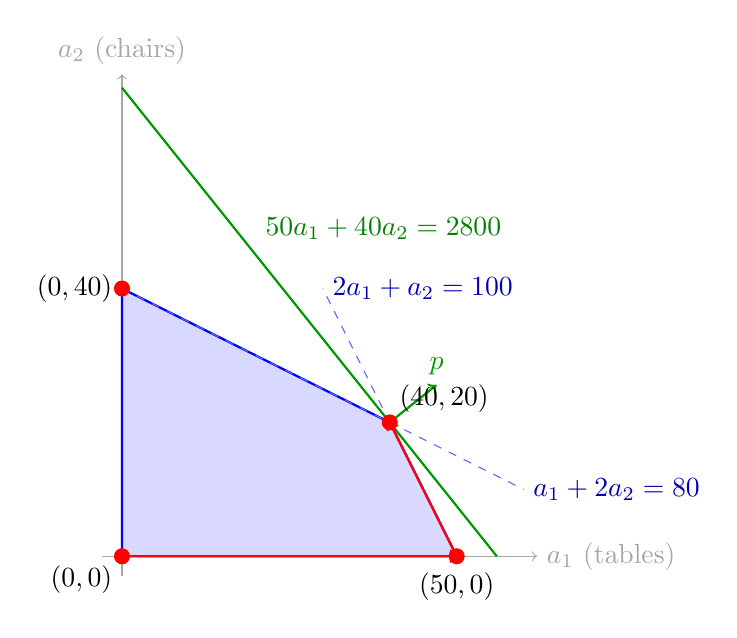
\begin{tikzpicture}[x=0.085cm, y=0.085cm]
			% Axes
			\draw[gray!70, ->] (-3,0) -- (62,0) node[right] {$a_1$ (tables)};
			\draw[gray!70, ->] (0,-3) -- (0,72) node[above] {$a_2$ (chairs)};

			% Feasible region with vertices (0,0), (50,0), (40,20), (0,40)
			\fill[blue!15] (0,0) -- (50,0) -- (40,20) -- (0,40) -- cycle;
			\draw[blue, thick] (0,0) -- (50,0) -- (40,20) -- (0,40) -- cycle;

			% Constraint lines extended
			\draw[blue!60, dashed] (50,0) -- (30,40);
			\draw[blue!60, dashed] (0,40) -- (60,10);
			\node[blue!70!black, right] at (30,40) {$2a_1 + a_2 = 100$};
			\node[blue!70!black, right] at (60,10) {$a_1 + 2a_2 = 80$};

			% Optimal objective level line 50a1 + 40a2 = 2800
			\draw[green!60!black, thick] (56,0) -- (0,70);
			\node[green!50!black, right] at (20,49) {$50a_1 + 40a_2 = 2800$};
			\draw[green!60!black, ->, thick] (40,20) -- (47,25.6) node[above] {$p$};

			% Simplex path
			\draw[red, thick, ->] (0,0) -- (50,0);
			\draw[red, thick, ->] (50,0) -- (40,20);

			% Vertices
			\foreach \p in {(0,0),(50,0),(40,20),(0,40)} \fill[red] \p circle (1.2);
			\node[below left] at (0,0) {$(0,0)$};
			\node[below] at (50,-1) {$(50,0)$};
			\node[above right] at (40,20) {$(40,20)$};
			\node[left] at (0,40) {$(0,40)$};
		\end{tikzpicture}
		\caption{The feasible region of the furniture problem. Simplex starts at the origin and moves along edges (red) to the vertex $(40,20)$, where the objective level line (green) touches the region last.}
	\end{figure}

\subsection{Interior-Point Methods and the Lagrangian View}

	Simplex walks along the boundary of $P$. Interior-point methods instead travel through its interior. Replace the standard-form LP by the barrier problem 
	\begin{equation}
		\min_{x} \; cx - \mu \sum_{j=1}^n \log x_j \quad \text{s.t.} \quad Ax = b, 
	\end{equation}
	for $\mu > 0$. The logarithm forces $x > 0$, so the solution $x(\mu)$ is interior. The optimality conditions of this strictly convex problem are 
	\begin{equation}
		Ax = b, \qquad A^\top \lambda^\top + s = c^\top, \qquad x_j s_j = \mu \;\; \forall j, \qquad x, s > 0, 
	\end{equation}
	with the sign convention that $s = c^\top - A^\top \lambda^\top \geq 0$ is the dual slack. The curve $\mu \mapsto (x(\mu), \lambda(\mu), s(\mu))$ is the \textbf{central path}. For $\mu = 0$ these conditions are exactly primal feasibility, dual feasibility and \textit{complementary slackness} $x_j s_j = 0$, so as $\mu \to 0$ the central path converges to an optimal primal-dual pair. Interior-point methods apply Newton's method to this system while decreasing $\mu$, and they take polynomially many Newton steps. The duality gap along the path is 
	\begin{equation}
		cx - \lambda b = x^\top s = n\mu, 
	\end{equation}
	which gives a certificate of how far we are from optimal at every iteration. 

	Finally, LP duality is a special case of Lagrangian duality, which is developed for general constrained problems in later sections. For the canonical primal, define the Lagrangian $L(a, \lambda) = pa + \lambda(r - Wa)$ for $a \geq 0$ and $\lambda \geq 0$. For fixed $a \geq 0$, 
	\begin{equation}
		\inf_{\lambda \geq 0} L(a, \lambda) = \begin{cases} pa & Wa \leq r \\ -\infty & \text{otherwise,} \end{cases}
	\end{equation}
	so $S = \sup_{a \geq 0} \inf_{\lambda \geq 0} L(a, \lambda)$. On the other hand, rearranging $L(a, \lambda) = \lambda r + (p - \lambda W)a$, for fixed $\lambda \geq 0$ 
	\begin{equation}
		\sup_{a \geq 0} L(a, \lambda) = \begin{cases} \lambda r & \lambda W \geq p \\ +\infty & \text{otherwise,} \end{cases}
	\end{equation}
	so $s = \inf_{\lambda \geq 0} \sup_{a \geq 0} L(a, \lambda)$. Weak duality is the general inequality $\sup \inf \leq \inf \sup$, and strong duality says that this minimax inequality is an equality for LPs, i.e. that $(a^\ast, \lambda^\ast)$ is a saddle point of $L$. Complementary slackness is then the statement that $L(a^\ast, \lambda^\ast) = pa^\ast = \lambda^\ast r$. 
